% Final report, NSF Future Manufacturing Data Challenge.
% 10pt sans-serif (Arial-equivalent), 1-inch margins, <= 3 pages.
\documentclass[10pt]{article}
\usepackage[margin=1in]{geometry}
\usepackage[T1]{fontenc}
\usepackage{helvet}
\renewcommand{\familydefault}{\sfdefault}
\usepackage{amsmath,amssymb}
\usepackage{graphicx}
\usepackage{booktabs}
\usepackage[font=normalsize,labelfont=bf]{caption}
\usepackage{titlesec}
\titlespacing*{\section}{0pt}{7pt}{3pt}
\setlength{\parskip}{2pt}
\setlength{\parindent}{0pt}
\pagestyle{empty}

\title{\vspace{-1.4em}\large\textbf{Predicting local laser-track geometry from in-situ
melt-pool thermal sequences}\vspace{-0.4em}}
\author{\normalsize Final report, NSF Future Manufacturing Data Challenge
(dataset arXiv:2607.07965)\\
\normalsize Development tracks 8/10/14; held-out test track 21}
\date{}

\begin{document}
\maketitle\thispagestyle{empty}
\vspace{-2.2em}

\section{Problem setup}
We work on a 0.2\,mm grid along the scan coordinate $x$ over the common
20--100\,mm window (400 positions per track, matching the 0.2\,mm/frame
spacing of the 50\,fps thermal stream). Given thermal frames $T$ and the
position $x$, we predict a vector $g(x)$ of local geometry descriptors as
five conditional quantiles,
\begin{equation}
\hat{F}^{-1}_{g(x)}(q \mid T_{x-k:x+k},\, x), \qquad
q \in \{0.05,\, 0.25,\, 0.50,\, 0.75,\, 0.95\},
\end{equation}
where $g$ contains the width $w(x)$, the boundaries $y_L(x)$, $y_R(x)$, the
center $c(x)$, edge roughness, waviness, contour deviation, peak relief,
cross-sectional area, and the profile $z(y \mid x)$. Height maps are used
for targets only; every model input is either measured during the scan or
is the coordinate $x$. All settings below were fixed by leave-one-track-out
(LOTO) cross-validation on the development tracks before track 21 was
evaluated once.

\section{Targets from the height maps}
The remelted track is optically smooth while the machined substrate is
rough, so the interferometer returns dense valid data inside the track and
sparse data outside. The per-$y$ valid-pixel fraction $v(y)$ within a bin
is therefore close to binary. With the threshold
\begin{equation}
\tau = \tfrac{1}{2}\left(P_{10}[v] + P_{90}[v]\right),
\end{equation}
the boundaries $[y_L, y_R]$ are the sub-pixel edges of the largest run
$\{y : v(y) > \tau\}$, giving $w = y_R - y_L$ and $c = (y_L + y_R)/2$, with
per-bin checks on contrast, width range, edge contact, and coverage. This
keeps 362 of 400 track-21 bins despite the partial profilometry failure on
that track. Writing $S_L$ for a moving-average smoother of window $L$ and
$b \in \{y_L, y_R\}$ for a boundary series,
\begin{equation}
r(x) = \operatorname{std}_{\pm 1\text{mm}}[\,b - S_{2}b\,], \quad
\omega(x) = \operatorname{std}_{\pm 5\text{mm}}[\,S_{2}b - S_{10}b\,], \quad
d(x) = \left|\, b - (\alpha + \beta x) \,\right|,
\end{equation}
averaged over both edges (roughness, waviness, and deviation from a
per-track linear toolpath fit). Cross-sections are detrended per bin with a
linear fit to the two substrate margins before we extract the peak relief
$h_{p90}$ and the area $A = \int z\, dy$.

\section{Thermal features and the isotherm anchor}
For each frame $f$ ($400 \times 400$ px, 14\,\textmu m/px) we compute
melt-pool descriptors (area, robust extents, elongation, centroid,
cooling-tail energy, scan asymmetry) with $\pm 0.4$ and $\pm 2$\,mm rolling
statistics, and the cross-track extent of the $c$-count isotherm,
\begin{equation}
E_c(x) = \Delta_{\mathrm{px}}\left(\max \mathcal{J}_c - \min \mathcal{J}_c\right),
\qquad
\mathcal{J}_c = \{\, j : \exists\, i,\ f_{ij}(x) > c \,\},
\end{equation}
for $c \in \{1300, \ldots, 1800\}$. The deposited width is set by the
solidification isotherm, so at the right count $E_c$ should track width
independently of laser power. On the development tracks the ratio
$w/E_{1400}$ is 0.887, 0.839, and 0.831 (CV 2.9\%; picking $c$ by minimum
ratio CV over the development tracks selects $c^{*} = 1400$). The anchor is
\begin{equation}
a(x) = k^{*}\, \bar{E}_{1400}(x), \qquad
k^{*} = \tfrac{1}{3} \sum_{t \in \mathrm{dev}}
\frac{\operatorname{med}[w_t]}{\operatorname{med}[\bar{E}_{1400,t}]} = 0.853,
\end{equation}
where $\bar{E}$ is the $\pm 2$\,mm rolling mean. Track 21 sits far outside
the development range (hot area 0.027 vs.\ 0.28--0.46\,mm$^2$); trees
saturate there, a linear anchor does not.

\section{Residual quantile model, calibration, and testing}
The width model keeps the extrapolating level separate from the learned
part:
\begin{equation}
\hat{w}_q(x) = a(x) + G_q\!\left(\phi(x)\right), \qquad
G_q = \arg\min_{G} \sum_{x \in \mathrm{dev}}
\rho_q\!\left(w(x) - a(x) - G(\phi(x))\right),
\end{equation}
where $\phi(x)$ stacks the thermal descriptors and $G_q$ is a
gradient-boosted tree ensemble (150 trees, depth 2, LOTO-selected) trained
with the pinball loss $\rho_q(u) = u\,(q - \mathbf{1}[u<0])$; predicted
quantiles are sorted. Feeding $a(x)$ to a standard GBM as one more feature
does not work (MAE 0.260\,mm), because trees cannot extrapolate below their
training range; the split in (6) is what makes the anchor useful. The level
uncertainty for an unseen power setting is estimated from the three LOTO
fold errors $e_j = \operatorname{med}[w] - \operatorname{med}[\hat{w}_{0.5}]$,
$s = \operatorname{RMS}(e_j) = 0.052$\,mm, and folded into the quantiles:
\begin{equation}
\tilde{Q}(q) = Q(0.5) + \operatorname{sign}(z_q)
\sqrt{\left(Q(q) - Q(0.5)\right)^2 + \left(z_q\, s\right)^2},
\qquad z_q = \Phi^{-1}(q).
\end{equation}
We score with MAE, 90\% interval coverage, and a CRPS approximation,
\begin{equation}
\mathrm{CRPS} \approx \tfrac{2}{q_{\max} - q_{\min}}
\int_{q_{\min}}^{q_{\max}} \rho_q\!\left(y - Q(q)\right) dq
\quad \text{(trapezoid over the five quantiles)} .
\end{equation}
Models are compared with a paired moving-block bootstrap of per-bin
absolute errors (block $= 25$ bins $= 5$\,mm, 2000 resamples). The
criterion, fixed in advance: a contribution counts as confirmed only if
the 95\% CI lower bound of $\Delta$MAE is above zero and the relative
improvement is at least 5\%. The anchor idea carries over to the height
direction, $h_{p90} \approx k_h \bar{E}_{1400} + G(\phi)$ with
$k_h = 7.27$\,\textmu m/mm and $A \approx k_a \bar{E}_{1400}^2 + G(\phi)$
with $k_a = 3.39$. Full cross-sections use a functional PCA fitted on the
development tracks,
\begin{equation}
z(u \mid x) \approx \mu(u) + \sum_{k=1}^{3} c_k(x)\, \varphi_k(u),
\qquad u = \tfrac{y - y_L}{w} \in [0, 1],
\end{equation}
with the coefficients $c_k(x)$ regressed from $\phi(x)$.

\section{Results (one frozen track-21 evaluation, 362 bins)}
\begin{table}[h]
\centering
\begin{tabular}{lllll}
\toprule
Descriptor & MAE (best) & vs.\ x-only & 90\% cov. & Verdict \\
\midrule
Width $w(x)$ & 0.089 mm & $-75.6\%$, CI $[0.246, 0.305]$ mm & 0.88 & confirmed \\
Boundaries $y_L$ / $y_R$ & 0.092 / 0.067 mm & $-58\%$ / $-62\%$ & -- & confirmed \\
Waviness $\omega(x)$ & 0.0035 mm & $-39\%$ & 0.93 & confirmed \\
Peak relief $h_{p90}$ & 2.15 \textmu m & $-55\%$ (tree 3.17) & 0.77 & confirmed \\
Area $A(x)$ & 0.96 \textmu m$\cdot$mm & $-67\%$ (tree 2.04) & 0.90 & confirmed \\
Center $c(x)$ & 0.062 mm & x-only already best & 0.98 & no thermal gain \\
Edge roughness $r(x)$ & 0.0132 mm & no gain, either modality & 1.00 & not predictable \\
Contour deviation $d(x)$ & 0.0184 mm & $\approx$ global median & 0.91 & not predictable \\
Profile $z(y \mid x)$ & 2.42 \textmu m & shape modes fail dev-LOTO & -- & amplitude only \\
\bottomrule
\end{tabular}
\end{table}
\vspace{-0.6em}
\begin{figure}[h]
\centering
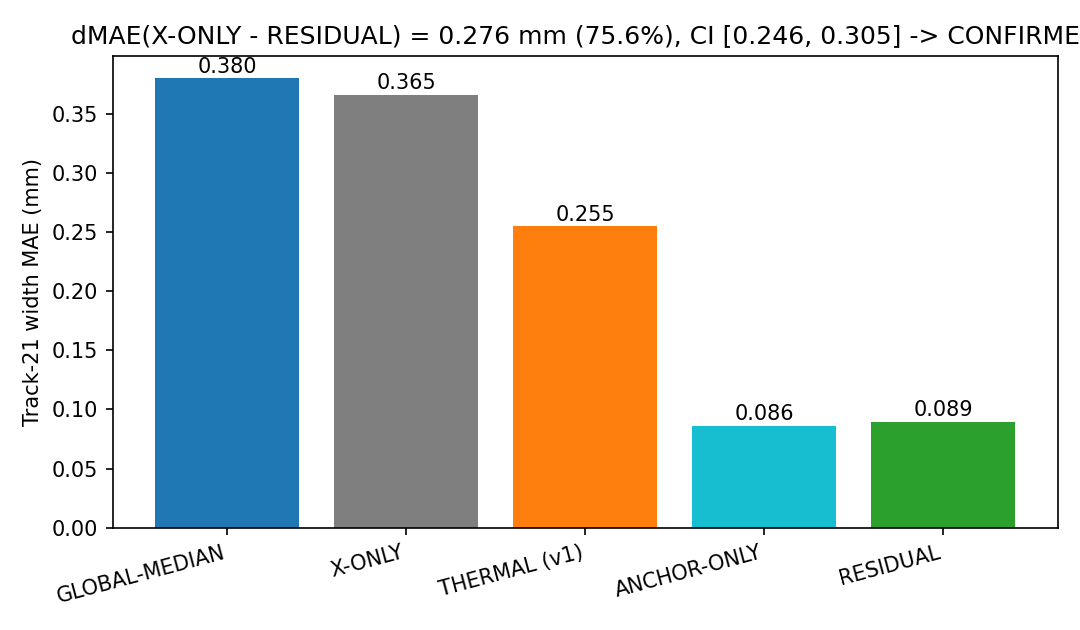
\includegraphics[width=0.44\textwidth]{figures/final_track21_mae_ladder_v2p1.png}\hfill
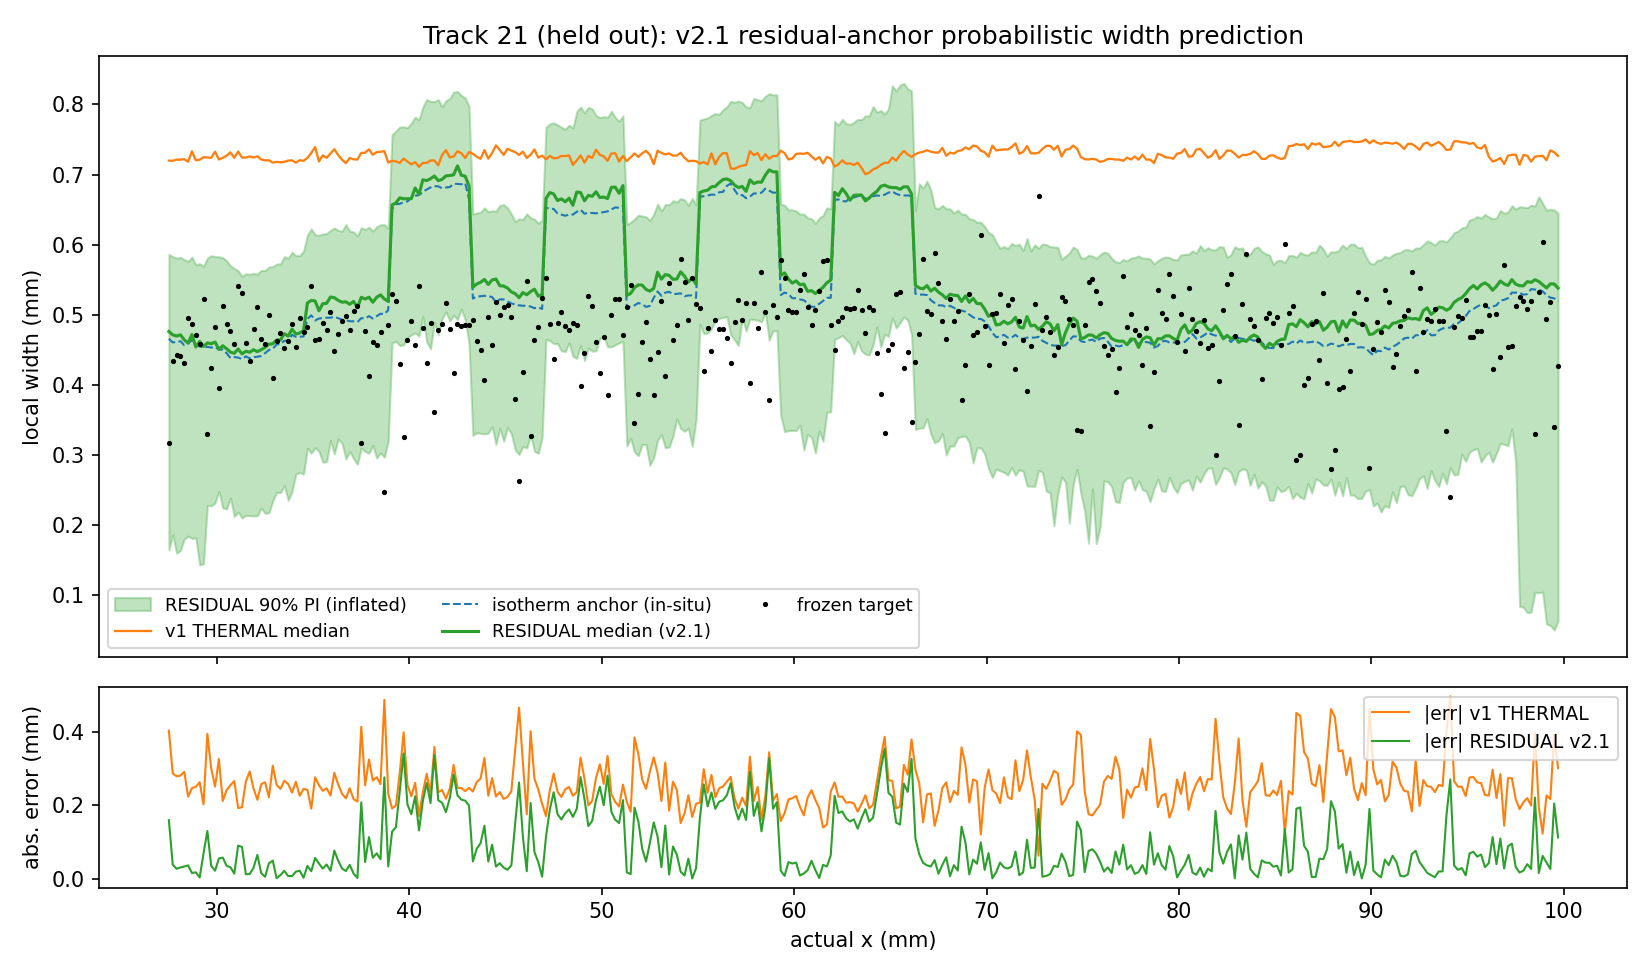
\includegraphics[width=0.54\textwidth]{figures/final_track21_predictions_v2p1.png}
\caption{Left: track-21 width MAE by model; the anchor (5)--(6) removes the
0.25\,mm level bias that pure tree models carry across the power gap.
Right: predictions along the track with the 90\% interval from (7).}
\end{figure}

\section{Sources of variation and what the results mean}
The table splits local geometry by physical pathway. Quantities driven by
the melt-pool thermal history ($w$, $y_L$/$y_R$, $\omega$, $h_{p90}$, $A$)
are predicted well from in-situ data; the waviness gain fits a melt-pool
oscillation origin. The center line needs only $x$, which is what one would
expect for a toolpath-defined quantity. Edge roughness, contour deviation,
and the ripple-scale profile shape were not predictable from either
modality. We tested the substrate route directly with a substrate-only SEM
protocol (track band detected and masked with a $\pm 0.30$\,mm margin,
texture features taken from 1.0\,mm strips on both sides, band location
never used as a feature): no target passed the criterion. Width gained
$+1.6\%$ with CI $[0.0008, 0.0024]$\,mm, above zero but below the 5\% bar,
close to the 1.8\% unconfirmed SEM gain reported by an independent baseline
on the same data.

Three points summarize the interpretation. First, one physical quantity
does most of the work: the ratio $w/E_{1400} \approx 0.85$ holds across a
$2\times$ power range, which points to the solidification isotherm as the
mechanism that sets the width. Second, model structure matters as much as
the feature itself: the same anchor fails as a tree input and works in the
residual form (6). Third, the remaining along-track fluctuation appears
information-limited rather than model-limited: within-track thermal--width
correlations stay below $|r| = 0.35$, predicting the shape modes in (9) is
worse than a constant mean shape even in development LOTO (2.04 vs.\
1.89\,\textmu m), and the rank-3 reconstruction floor of 0.41\,\textmu m
bounds what perfect coefficients would give. A CNN on the same inputs would
face the same limit with 1{,}122 training rows over three power settings.

\section{Limitations}
Three power settings make every cross-condition calibration thin. The
height anchor over-predicts in the near-threshold 200\,W regime, where the
relief scaling is no longer linear. The isotherm idea was checked coarsely
on all four tracks before the freeze; all frozen constants come from the
development tracks, but a pre-registered replication on new tracks would
be the cleaner test. Scan orientation per track is inferred from
development data rather than documented. Finally, results depend on the
label definition: replicating the method inside the baseline repository
showed that its gradient-edge labels are nearly power-invariant (0.741 to
0.804\,mm from 200 to 400\,W), and under that definition the anchor is
correctly rejected by the same criterion, while it is confirmed
(70.1\% improvement) under the validity-run labels used here. The full
pipeline, frozen configuration files, hashes, and a single reproduction
command accompany this report.

\end{document}
